\documentclass[a4paper]{article}
\usepackage[italian]{babel}
\usepackage[utf8]{inputenc}
\usepackage{amssymb,amsmath,amsfonts}
\usepackage{graphicx}
\usepackage{listings}

\lstset{basicstyle=\scriptsize\tt} 

\author{Guido De Rosa}

\begin{document}

\title{Ricerca degli zeri di una funzione con il metodo delle secanti}

\maketitle

%% \section{Introduzione}

Si cercano gli zeri della funzione
\[
  \cos{\exp{x}} + \sin{2x} - \frac{7}{200} 
\]
nell'intervallo $(-8, 2)$. Agli estremi di tale intervallo la funzione
assume segni diversi, dunque per continuità deve esserci \emph{almeno}
uno zero. Adoperando il metodo delle secanti, partendo proprio dagli estremi,
possiamo trovarne uno. 

In \texttt{lib/zero/secant.rb} c'è un iteratore che implementa il metodo 
delle secanti:
\begin{lstlisting}
    def each
      while
          f(@upper) * f(@lower) < 0           and
          value.abs > @epsilon                and
          @steps < @maxsteps
        yield @lower, @upper, @pivot, value()
        @pivot = @lower - f(@lower) * (@upper-@lower) / (f(@upper)-f(@lower))
        if f(@pivot)*f(@lower) < 0
          @upper = @pivot
        elsif f(@pivot)*f(@upper) < 0
          @lower = @pivot
        end
      end
      yield @lower, @upper, @pivot, value()
    end
\end{lstlisting}

Questo metodo è invocato nello script \texttt{single\_interval\_demo.rb},
che illustra lo stato di ogni passaggio fino al raggiungimento di un zero
(cioè di un punto in cui $|f(x)| < \epsilon$, con $\epsilon$ ``piccolo''
qui convenzionalmente scelto $\epsilon = 10^{-12}$).

L'output del programma è:
\begin{lstlisting}
In [-8.0..2.0], f(-3.0) = 1.243176378098289
In [-0.15144772809181362..2.0], f(-0.15144772809181362) = 0.3195593828610368
In [0.8855197885517707..2.0], f(0.8855197885517707) = 0.19146677651610636
In [0.8855197885517707..1.284436849096858], f(1.284436849096858) = -0.38417753797427334
In [0.8855197885517707..1.018204784750278], f(1.018204784750278) = -0.07255630929479703
In [0.8855197885517707..0.9817415580843608], f(0.9817415580843608) = -0.0015526630636658323
In [0.8855197885517707..0.9809675428463149], f(0.9809675428463149) = -1.963182664951879e-05
In [0.8855197885517707..0.9809577572234991], f(0.9809577572234991) = -2.447736079103091e-07
In [0.8855197885517707..0.9809576352145194], f(0.9809576352145194) = -3.0513440385515622e-09
In [0.8855197885517707..0.9809576336935574], f(0.9809576336935574) = -3.8037878402619185e-11
In [0.8855197885517707..0.9809576336745971], f(0.9809576336745971) = -4.741484982417887e-13
\end{lstlisting}
Come si vede, è stato trovato uno zero per $x \simeq 0.981$.

Esistono altri zeri?

Nello script \texttt{multi.rb} si suddivide l'intervallo $(-8, 2)$ 
in 32 sottintervalli ``random''\footnote{La suddivisione casuale di un intervallo è implementata in \texttt{lib/core/range.rb}.}, 
e si ripete la ricerca di un eventuale
zero in ciascuno di questi.
\begin{lstlisting}
@f        = lambda {|x| cos(exp(x)) + sin(2*x) - 0.035}
@interval = (-8.0..2.0)

@interval.randomly_partition(32) do |subinterval|
  zs = Zero::Secant.new(
    :lower => subinterval.first,
    :upper => subinterval.last,
    :f     => @f
  )
  x0 = zs.find and puts "#{x0} #{zs.value}"
end
\end{lstlisting}

Questo è l'output: sono elencate le coppie $(x, f(x))$ trovate in cui 
$|f(x)| < \epsilon$:
\begin{lstlisting}
-7.201260475389554 -8.813783036742961e-13
-6.935906094682003 -6.371292382567617e-13
-1.0113901440550748 -3.929911951416898e-13
-0.43323305742286206 -5.452027718177987e-13
0.9809576336748386 -9.524325772503062e-13
1.547909485194127 -9.077461005091436e-14
1.9519150433007135 3.344269305927128e-13
\end{lstlisting}

Non è detto che questo metodo trovi sempre tutti gli zeri, ma in questo
caso i risultati sembrano sodisfacenti, come si può vedere in 
Fig. \ref{fig:plot}.

\begin{center}
  \begin{figure}

    \begin{center}
      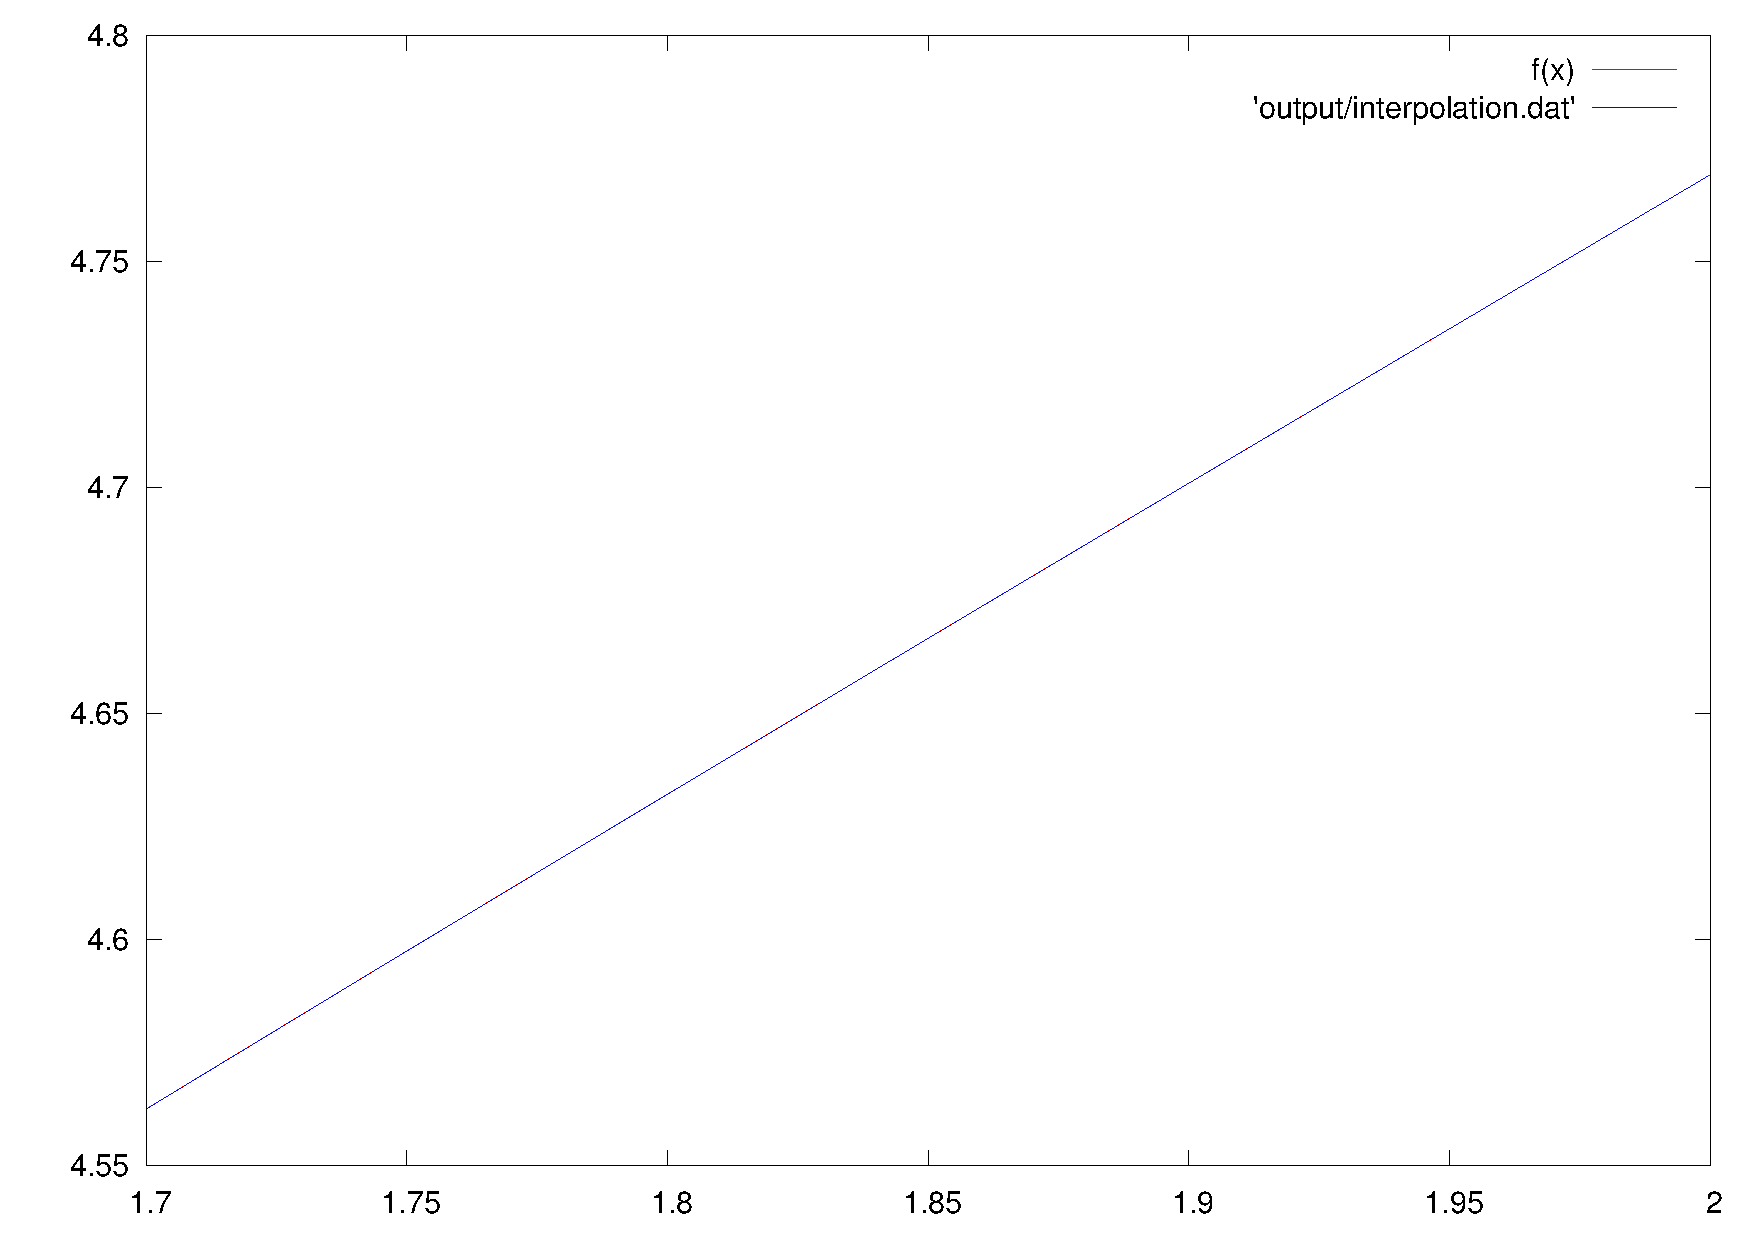
\includegraphics[width=130mm]{plot.pdf}
    \end{center}

    \caption{  }
    
    \label{fig:plot}
    
  \end{figure}
\end{center}

\end{document}
